
\chapter{Selección de componentes}
En este capítulo se procede a exponer las características mas importantes  de los componentes del sistema, así como las consideraciones y 
posibildades que tuvimos en cuenta en el proceso de selección de los mismos. \par

En el momento de comenzar este proyecto, rapidamente nos vimos ante la necesidad de seleccionar los componentes de nuestro sistema. 
En este proceso tuvimos en cuenta los objetivos y el diagrama de funcionamiento general que se trató en el capítulo de características que precede,
además de otras consideraciones como el costo, los conocimientos previos del equipo sobre el componente, disponibilidad, etc. 
Para poder explicar como fue este proceso, dividimos el sistema en tres etapas: Recepción, Procesamiento y alarmas, y comunicación.

\section{Etapa receptora de RF} \par
De acuerdo al plantemiento del sistema, una parte crucial en el funcionamiento del mismo es la recepción de la señal de interés.
Vale recordar que la etapa de recepción se encuentra presente en todos los nodos del sistema, por lo que las diferencias de costos
en este apartado se ven multiplicadas.\par
La recepción debe cumplir con las siguientes características:

\begin{itemize}
    \item Antena para 433MHz. Es el primer componente a tener en cuenta cuando hablamos de comunicaciones inalámbricas. En este caso, 
    este transductor nos servirá para obtener la energía electrica que podemos entender y analizar, a partir de la ondas electromagnéticas
    emitidas por la llave de automovil y por los inhibidores. Planteamos la posibilidad de utilizar dos tipos de antenas, del tipo 
    omnidireccional o una con la capacidad de generar un barrido, característica importante si se quiere obtener la posición del inhibidor.

    \item Demodulación de señales ASK en 433MHz. Es el principal requerimiento de la recepción debido a las características de las 
    comunicaciones presentes en los sistemas de seguridad de vehículos.

    \item Medición de RSSI. La medición del nivel de potencia de la señal recibida es crucial para poder identificar adecuadamente
    a los inhibidores. También cumple un rol indispensable en uno de los objetivos secundarios mas desafientes del sistema como lo es la obtención
    de la posición del elemento inhibidor mediante la triangulación.

    \item Comunicación con microcontrolador. Es importante tener en cuenta las posibilidades que nos ofrece esta etapa a la hora de comunicarse
    con la siguiente. Los datos obtenidos de la recepción de la señal serán procesados por un microcontrolador.

\end{itemize}

Luego de estudiar las mejores opciones llegamos a una que consiste en utilizar un esquema como el que vemos en la figura
\ref{EtapaReceptora1}. En primer lugar elegimos utilizar una antena omnidireccional, es la opción que nos permite reducir los precios
y simplificar el sistema al evitar sistemas de matrices antenas o antenas con rotación.
El inconveniente de esta elección, es que la antena omnidireccional no nos entrega informacion referida al angulo en que recibe la señal, por lo que
complica la obtención de la posición. Sin embargo, todavía es posible comparando la lectura del nivel de RSSI de cada nodo.
Luego encontramos un divisor de potencia de RF que se encarga de entregar la señal al demodulador ASK, y al medidor de potencia. \par

\begin{figure}[htb]
	\centering
	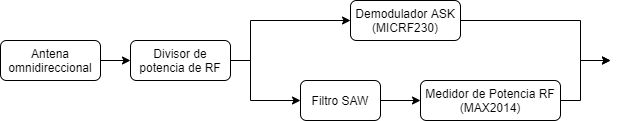
\includegraphics[scale=0.6]{images/Opcion1.png}
    \caption{Etapa receptora - primer opción}
	\label{EtapaReceptora1}
\end{figure}


Vemos que este diagrama cumple con las características anteriormente expuestas. Sin embargo, al final nos decantamos por otra opción, 
esta consiste en utlizar un módulo transceptor CC1101. La incorporación de este módulo, nos permite reducir mucho los costos y simplificar
el sistema sin sacrificar características importantes. \par
En la figura \ref{EtapaReceptora2} vemos como resulta el nuevo diagrama de la etapa receptora. \par

\begin{figure}[htb]
	\centering
	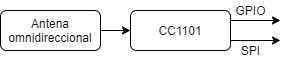
\includegraphics[scale=0.6]{images/Opcion2.png}
    \caption{Etapa receptora - opción elegida}
	\label{EtapaReceptora2}
\end{figure}

A simple vista podemos apreciar que se reducen la cantidad de componentes. Esto se debe a que el módulo CC1101 es capaz de demodular la señal y
entregar la secuencia de bits mediante un pin de GPIO, así como también medir la potencia de la señal y comunicar el valor mediante comunicación SPI.
La unica desventaja de esta opción es que el módulo posee peor rango de RSSI que un componente medidor de potencia específico para ese fin,
esto provoca que señales de gran potencia saturen nuestro receptor y nos imposibilite triangular de manera correcta, sin embargo la determacion 
de la posición es un objetivo secundario. \par
En la sección \ref{cap:cc1101} se exponen en detalle las características del módulo.\par

\section{CC1101} \label{cap:cc1101}
\subsection{Transceptor}
\subsubsection{Descripción del componente}


\begin{figure}[htb]
	\centering
	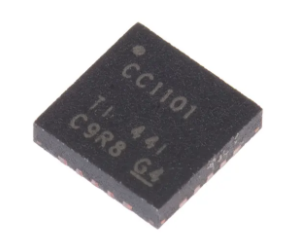
\includegraphics[scale=0.6]{images/CC1101.png}
    \caption{Transceptor CC1101}
	\label{fig:cc1101}
\end{figure}

CC1101 es un transceptor para frecuencia inferiores a 1GHz de bajo costo para aplicaciones inalámbricas de baja potencia. Está destinado principalmente
a aplicaciones ISM (industrial, científico y médico) y bandas de frecuencia SRD (Dispositivo de corto alcance) a 315, 433, 868 y 915Mhz, pero puedo ser programado 
para funcionar en otros bandas. EL transceptor RF está integrado con un módem de banda base configurable que admite varios formatos de modulación.\par 
CC1101 proporciona un amplio soporte de hardware para manejo de paquetes, almacenamiento en búfer de datos, transmisiones de ráfagas, evaluación de canal,
indicación de calidad de enlace y wake-on-radio. \par 
En un típico sistema, el CC1101 se utilizará junto con un microcontrolador y algunos componentes pasivos adicionales.

\subsubsection{Características generales}

En este apartado mostramos algunas caracteristicas importantes del CC1101 sin extendernos demasiado. Si se quiere mas información sobre este integrado ver \todo 

\begin{itemize}
    \item Alimentación de 3.3V
    \item Sensibilidad: 
    \subitem -116 dBm a 0.6kBaud en 433MHz
    \subitem -112 dBm a 1.2kBaud en 868 MHz
    \item Velocidad de datos: Hasta 250kbaud en ASK.
    \item Bajo consumo de corriente: 14.7mA en RX.
    \item Admite 2-FSK, 4-FSK, GFSK y MSK, así como OOK y ASK.
    \item Medición de RSSI entre -110dBm a -20dBm.
    \item Interfaz SPI, a través de la cual se puede configurar todos los registros.
    \item Filtro digital de banda ancha programable. 58-812kHz.
\end{itemize}

\subsection{Módulo}

El modulo aporta simplicidad al sistema, ya que contiene los componentes pasivos necesarios para el funcionamiento del CC1101. También permite mejor acceso a los pines 
del integrado y tiene conexión SMA para antena. En nuestro caso particular, este módulo fue necesario debido a que soldamos los componentes de forma manual y porque
tiene un gran disponibilidad en el mercado.

En la figura \ref{fig:sch_cc1101} podemos ver el esquemático del módulo y en la figura \ref{fig:module_cc1101} podemos ver el aspecto físico.

\begin{figure}[htb]
	\centering
	\includegraphics[scale=0.6]{images/EsquemáticoCC1101.jpg}
    \caption{Esquemático CC1101}
	\label{fig:sch_cc1101}
\end{figure}

Se puede observar en el esquemático, que el módulo es muy simple en cuanto a los componentes que posee. Pero aún así es muy util en nuestra aplicación.

\begin{figure}[htb]
	\centering
	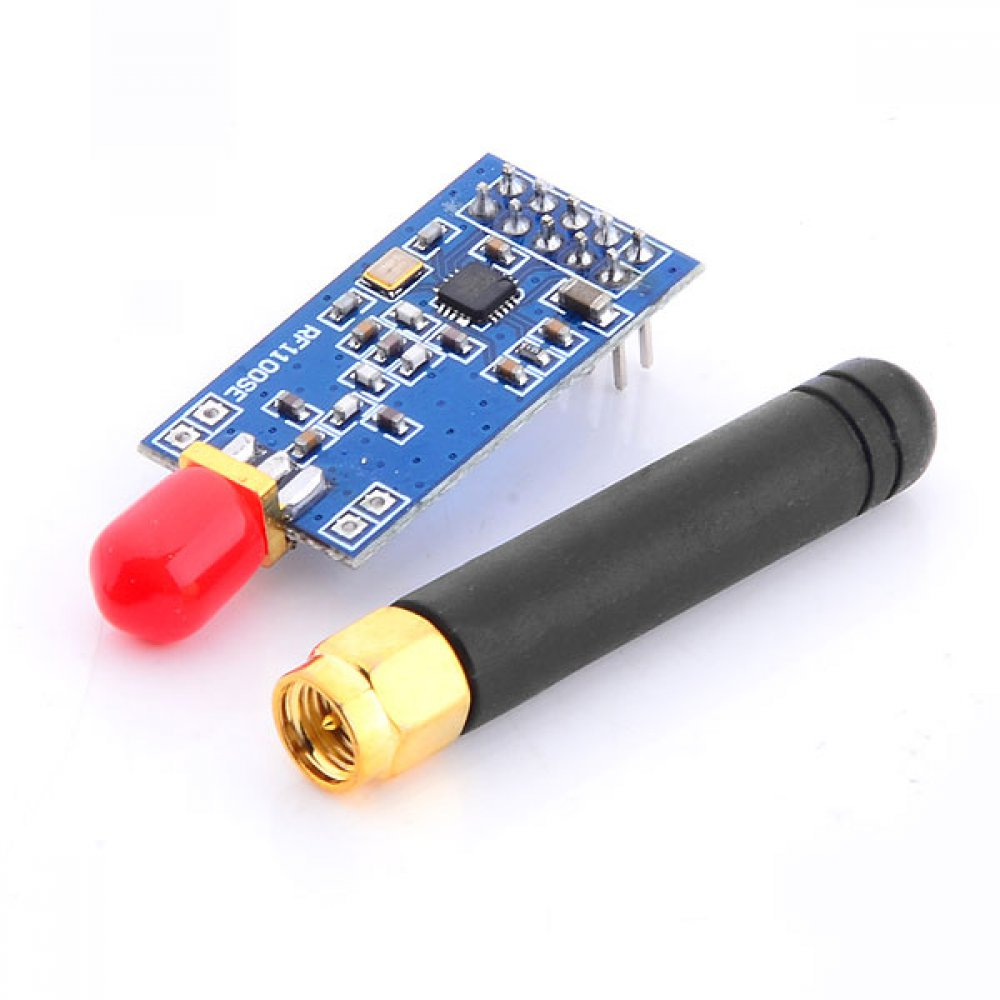
\includegraphics[scale=0.2]{images/modulo_cc1101.jpg}
    \caption{Módulo CC1101}
	\label{fig:module_cc1101}
\end{figure}

\section{Comunicación Serial}

La comunicación se puede dividir en dos partes, la primera referida a la comunicación entre los nodos y la central y la otra, referida a la comunicación
de la central con un servidor web.
\subsection{Comunicación local}

Según nuestros objetivos, la comunicación debe reunir las siguientes características:

\begin{itemize}
    \item Resistencia a ataques de inhibidores. Es importante que la comunicación local no sea vulnerable a los mismos ataques que intentamos identificar, ya que
    si fallara la comunicaciónn entre los nodos y la central el sistema no puede dar aviso de la presencia de una señal interferente.
    \item Comunicación bidireccional. Para establecer una red multinodal adecuada necesitamos un sistema de comunicación half-duplex o full-duplex, ya que 
    la central comandará a los nodos, los cuales le responden con la información que la central les requiere.
    \item Distancia mayor a 1000m. Es probable que el sistema sea instalado en lugares abiertos como estacionamientos, por lo que necesitamos un protocolo de 
    comunicación capaz de funcionar a largas distancias.
    \item Buena velocidad de comunicacion. No requerimos de velocidades muy altas, sin embargo es una característica a tener en cuenta.
    \item Cableado de bajo costo. Como ya mencionamos, es probable que la distancia entre nodos sea grande, por lo que el precio del cableado debe ajustarse 
    a nuestros objetivos.

\end{itemize}

Teniendo en cuenta las necesidades y analizando las opciones, determinamos que la mejor opción para nuestra aplicación es usar el estandar de comunicación RS485. 
Este está definido como un sistema de bus diferencial multipunto, ideal para transmitir a altas velocidades sobre largas distancias y a través de canales ruidosos.
El medio físico de transmisión es un par trenzado con una longitud máxima de 1200 metros operando entre 300 y 19200 bit/s y la comunicación semiduplex.\par
Las especificaciones de este estandar son:

\begin{itemize}
    \item Interfaz diferencial
    \item Conexión multipunto
    \item Alimentación de 5V
    \item Hasta 32 estaciones 
    \item velocidad Máxima de 10Mbit/s (a 12 metros)
    \item Longitud máxima de alcance de 1200 metro (a 100kbit/s)
    \item Rango de bus de -7V a +12V

\end{itemize}

Para nuestra aplicación usaremos el RS485 en combinación de la UART de nuestro microcontrolador, por lo que necesitaremos utilizar un transceptor MAX485 
(ver sección \ref{cap:max485}). Utilizaremos uno en cada nodo y en la central. El MAX485 tiene la capacidad de transformar los datos de la UART al estandar
RS485 y viceversa. \par

\subsection{Comunicación con Servidor Web}

Una de las características mas importantes del proyecto, es la capacidad de subir la información a un Servidor Web, por lo que es indispensable que la central disponga
de conexión a internet.\par
Debido a que no podemos asegurar que en el lugar donde se instale el sistema cuente con conexión a internet cableada o WiFi, decidimos utilizar conexión GSM mediante 2G. \par
En el mercado podemos encontrar varios módulos para conexiones GSM/GPRS. En la tabla \ref{tab:gsm} podemos ver algunas opciones.

\begin{table}[t]
    \begin{center}
        \begin{tabular}{ | m{3cm} | m{3cm} | m{3cm} | m{3cm} | }
        \hline Módulo & SIM800L & SIM900 & A6  \\ \hline
        Velocidad de transmisión & 1200 bp - 115200 bp. & 1200bp - 115200bp. & 1200bp - 115200bp. \\ \hline
        Tensión de operación & 3.4V - 4.4V & 9V - 20V & 3.3V - 4.2V \\ \hline
        Corriente & Hasta 2A & Hasta 2A & Hasta 2A\\ \hline
        Comunicación & Comunicación serial &Comunicación UART & Comunicación serial\\ \hline
        Precio & 13,39 usd &  48,70 usd & 18,26 usd\\ \hline
        
        \end{tabular}
        \caption{Módulos GSM disponibles en el mercado}
        \label{tab:gsm}   
    \end{center}
\end{table}

Nosotros elegimos el módulo sim800l por dos razones, la primera es el bajo precio comparado con el sim900 y la segunda por la experiencia previa
que disponíamos con este módulo.
En la sección \ref{cap:sim800l} se detallan las características de este componente.

\section{MAX485} \label{cap:max485}

MAX 485 es un transceptor de baja potencia para comunicación RS-485 y RS-422. Cada integrado contiene un controlador y un receptor.\par 
La velocidad de respuesta del controlador del MAX485 no está limitada, lo que les permite transmitir hasta 2,5 Mbps. Estos transceptores
consumen entre 120 µA y 500 µA de corriente de suministro cuando están descargados o completamente cargados con controladores desactivados.
Todas las piezas funcionan con un solo suministro de 5V. 

\begin{figure}[htb]
	\centering
	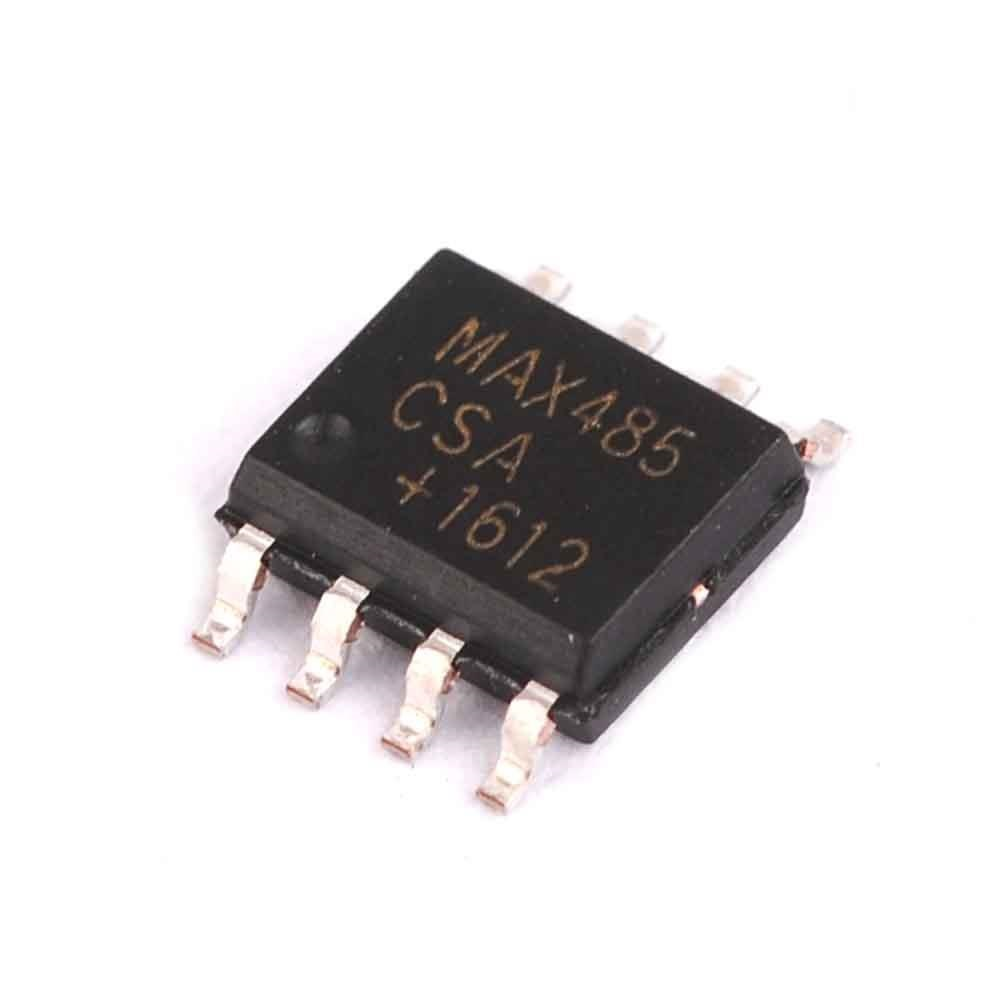
\includegraphics[scale=0.5]{images/max485.jpg}
    \caption{Max 485}
	\label{fig:max485}
\end{figure}

Los controladores tienen limitación de corriente de cortocircuito y están protegidos
contra una disipación de energía excesiva mediante un circuito de apagado térmico que coloca las salidas del controlador en un estado de alta 
impedancia. La entrada del receptor tiene una característica a prueba de fallas que garantiza una salida lógica alta si la entrada está en 
circuito abierto. El MAX485 está diseñado para aplicaciones semidúplex.

\section{SIM800L} \label {cap:sim800l}

\subsection{Descripción del componente}

Utilizamos el SIM800L a través de un módulo del mismo nombre, como se suele utilizar normalmente. El módulo nos permite accesar a los pines 
mas importantes del SIM800L para manejarlo desde un microcontrolador.\par
Consiste en un módulo cuatribanda que permite agregar funcionalidades avanzadas de comunicación a través de la red celular, como mandar mensajes de texto,
datos o realizar llamadas en un tamaño sumamente compacto. 

\begin{figure}[htb]
	\centering
	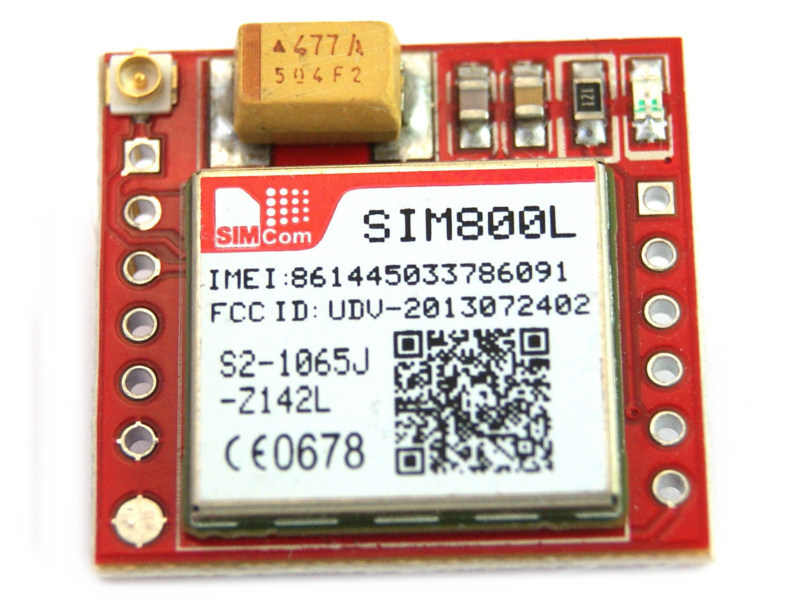
\includegraphics[scale=0.2]{images/sim800l.png}
    \caption{Módulo SIM800L}
	\label{fig:sim800l}
\end{figure}

\subsection{Caracteísticas Generales}

A continuación se listan algunas características importantes de este módulo. Sin embargo, si se quiere ver en mayor profundidad ver \todo

\begin{itemize}
    \item Tensión de operación: 3.4V - 4.4V
    \item Nivel lógico de 3-5V
    \item Consumo de corriente:
    \subitem Máximo: 500mA con picos de 2A
    \subitem En reposo: 0,7mA
    \item Interfaz serial UART
    \item Quad-Band 850/900/1800/1900MHz. Conexión a cualquier red mundial por 2G.
    \item Controlado por comandos AT
    \item Velocidades de transmisión serial desde 1200bps hasta 115 200 bps
    \item Tamaño de la SIM: Micro SIM
\end{itemize}

\section{Procesamiento} \par

Tanto en los nodos como en la central, es indispensable el uso de un microcontrolador. En el caso del nodo, se encarga de comunicarse con la etapa receptora,
procesar la información y decidir si la señal recibida proviene de un inhibidor, luego debe ser capaz de comunicarse con el MAX485 para establecer la comunicación
RS485 con el resto del sistema. En la central, el microcontrolador es el encargado de recibir la información de nodos a través del MAX485 y,
en caso de la presencia de un inhibidor, activar las alarmas correspondientes y actualizar la información en el servidor web mediante el módulo sim800l. \par

El microcontrolador que utilizamos tanto para los nodos como en la central es el stm32f103c8t6. La decisión de utilizar este microncontrolador se tomó debido 
a sus características, el bajo precio y sobre todo porque ya contábamos con experiencia en su uso.
En este caso, decidimos utilizar un módulo de desarrollo llamado "Blue Pill". Las características de esta placa la podemos ver en la sección \ref{cap:bluepill}

En la tabla \ref{tab:uC} podemos ver una comparación entre nuestro microcontrolador y otras opciones similares de otros marcas.

\begin{table}[t]
    \begin{center}
        \begin{tabular}{ | m{3cm} | m{3cm} | m{3cm} | m{3cm} | }
        \hline  & Blue Pill & Arduino Nano & PIC18F4520  \\ \hline
        Procesador & ARM 32 bits & AVG 8bits & PIC 8bits \\ \hline
        Frecuencia de Funionamiento & 72MHz &20MHz & 8MHz \\ \hline
        Memoria FLASH & 64 o 128kb & 32kb & 32kb\\ \hline
        SRAM & 20Kb & 2Kb & 2Kb \\ \hline
        comunicacion & USB. SPI. I2C. USARTs &  USB. SPI. I2C. USARTs & EUSART. SPP. USB. SPI. I2C\\ \hline
        Precio & 6,20 usd &  6,67 usd & 13,39 usd\\ \hline
        
        \end{tabular}
        \caption{Comparación de microcontroladores}
        \label{tab:uC}   
    \end{center}
\end{table}

Es importante añadir que podemos programar la Blue Pill mediante un programador stlink v2, que tiene precio bajo comparado a otros programadores, y
utilizar el programa STM32CubeIDE del fabricante para debuggear el sistema, característica que fue muy importante en el desarrollo del proyecto.\par
En la sección \ref{cap:stm32} ahondamos mas sobre este módulo y el microcontrolador en cuestión. 

\section{Blue Pill STM32} \label{cap:stm32}
\subsection{stm32f103c8t6}

Es un microcontrolador perteneciente a la linea de rendimiento medio de la familia STM. Incorpora el npucleo RISC ARM Cortex de 32 bits de alto rendimiento,
posee memorias integradas de alta velocidad y una amplia gama de entradas y salidas. Este dispositivo ofrece dos ADC de 12bits, tres temporizadores de 16bits
de uso general mas un temporizador PWM, asi como diversas interfaces de comunicación.\par 
Este microcontrolador es apto para gran variedad de aplicaciones, como unidades de motor, control de aplicaciones, equipos médicos y portátiles, periféricos
de PC y juegos, plataformas GPS, aplicaciones industriales, PLC, inversores, impresoras, escáneres. , sistemas de alarma, videoporteros y HVAC.

A continuación se listan algunas de las características que nos parecen mas importantes de este microcontrolador:

\begin{itemize}
    \item Tensión de operación: 2 a 3,6V
    \item Frecuencia de 72MHz
    \item Memorias integradas de alta velocidad
    \subitem Memoria Flash de 128Kbytes
    \subitem Memoria SRAM de hasta 20Kbytes
    \item Interfaces de comunicación: Dos I2C y SPI, tres USART, un USB y un Candiani
    \item 37 GPIOs
    \item Dos ADC de 10 canales.
\end{itemize}

\subsection{Módulo Blue Pill} \label{cap:bluepill}

En nuestro sistema utilizamos la placa de desarrollo llamaba Blue Pill. Esta placa incorpora al stm32f103c8t6 y aporta los componentes pasivos
adecuados para su uso, también incorpora dos cristales, entrada microUSB, leds indicadores, boton de reset e integrado para regulación de tensión. \par
Incorporar esta placa simplifica el diseño de nuestros PCB, ya que nos facilita el acceso a los pines del microcontrolador y posibilita la conexión
con el programador, además nos permite desarrollar un proyecto donde soldemos de forma manual los componentes, reduciendo costos.\par
En la figura \ref{fig:sch_bluepill} vemos el esquemático de esta placa.

\begin{figure}[htb]
	\centering
	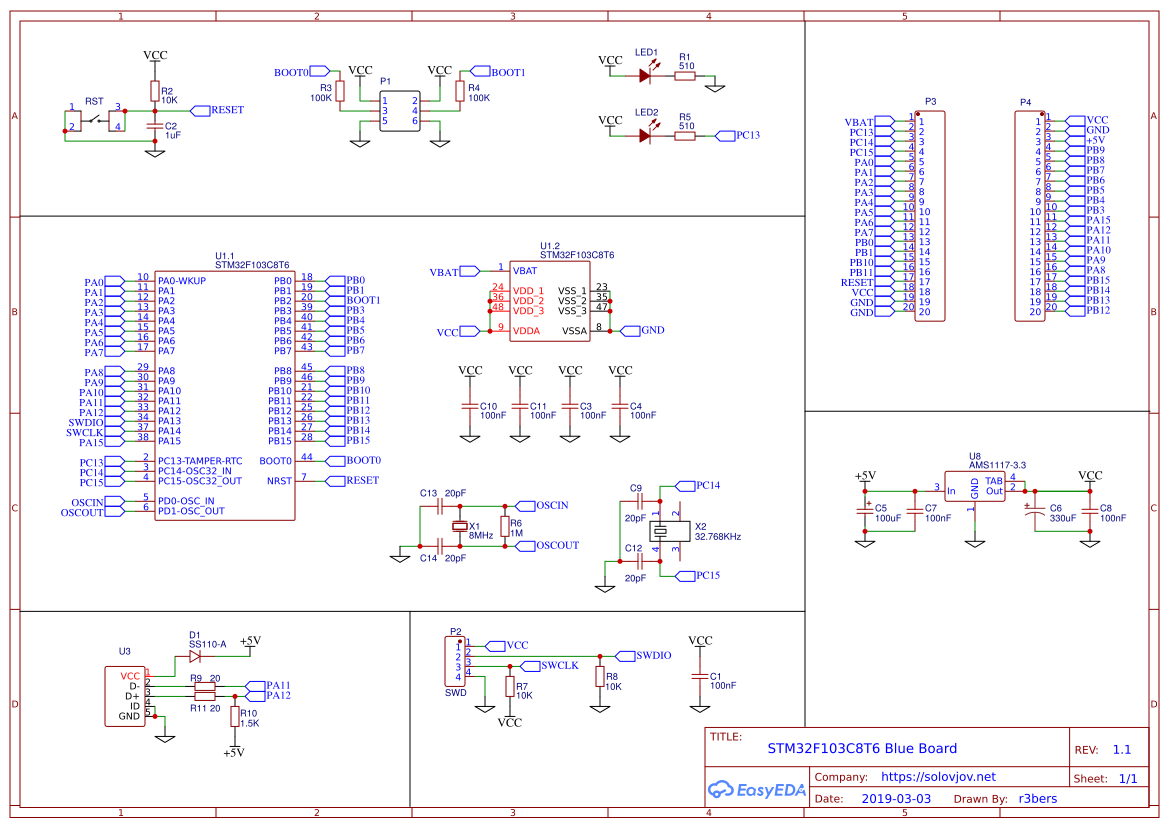
\includegraphics[scale=0.4]{images/esquematico_bluepill.png}
    \caption{Esquemático de Blue Pill}
	\label{fig:sch_bluepill}
\end{figure}
